% Uebungsaufgaben zur Vorlesung MoSi 3
% Blatt 1

\NeedsTeXFormat{LaTeX2e}
\documentclass[11pt,a4paper]{article}
%%%%%%%%%%%%%%%%%%%%%%%%%%%%%%%%%%%%%%%%%%%%%%%%%%%%%%%%%%%%%%%%%%%%%%%%%%%%%%%%
% Header fuer Uebungszettel                                                    %
% Jochen Siehr                                                                 %
% 2010-10-27                                                                   %
% last-change 2010-12-20                                                       %
%%%%%%%%%%%%%%%%%%%%%%%%%%%%%%%%%%%%%%%%%%%%%%%%%%%%%%%%%%%%%%%%%%%%%%%%%%%%%%%%

\usepackage{german}
\usepackage[T1]{fontenc}
\usepackage[utf8]{inputenc}

\usepackage{geometry}
\usepackage{amsmath,amsthm,amssymb}
\usepackage{epsfig}
\usepackage{setspace}
\usepackage{longtable}
\usepackage{enumerate}
\usepackage{eurosym}
\usepackage{siunitx}
\usepackage{pifont}
\usepackage{color}

\usepackage[ % letztes Paket!
 linkbordercolor={1 1 1},
 citebordercolor={1 1 1},
 menubordercolor={1 1 1},
 filebordercolor={1 1 1},
 urlbordercolor={1 1 1},
 pdfborder={0 0 0},
 pdftitle={Uebungsblatt},
 pdfauthor={Jochen Siehr}
 ]{hyperref}
\usepackage{breakurl} %muss danach kommen: AUSKOMMENTIEREN für pdflatex 

\pagestyle{empty}
\geometry{margin=20mm}
\setlength{\parindent}{0em}


\newcommand{\R}{\mathbbm{R}}
\newcommand{\C}{\mathbbm{C}}
\newcommand{\N}{\mathbbm{N}}
\newcommand{\Z}{\mathbbm{Z}}

\newcommand{\CC}{\mathbb{C}}
\newcommand{\NN}{\mathbb{N}}
\newcommand{\QQ}{\mathbb{Q}}
\newcommand{\RR}{\mathbb{R}}
\newcommand{\ZZ}{\mathbb{Z}}

\newcommand{\CCC}{\mathcal{C}}
\newcommand{\NNN}{\mathcal{N}}
\newcommand{\LLL}{\mathcal{L}}
\newcommand{\OOO}{\mathcal{O}}

\newcommand{\T}{\mathrm{T}}
\newcommand{\eqqcolon}{=\mathrel{\mathop:}}
\newcommand{\coloneqq}{\mathrel{\mathop:}=}

\newcounter{blatt}
\newtheoremstyle{jochen}{}{}{}{}{\bfseries}{}{\newline}{}
\theoremstyle{jochen}
\newtheorem{aufg}{Aufgabe}[blatt]
\newtheorem{loes}{L\"osungsskizze}[blatt]
\newtheorem{ex}{Exercise}[blatt]
\newtheorem{sol}{Solution}[blatt]



\newcommand{\tstep}{\Delta t}
\newcommand{\tend}{t_{\mathrm{end}}}
\newcommand{\bigO}{\mathcal{O}}
\newcommand{\quoterat}{\hspace{\fill}\qed}
\newcommand{\zB}{z.\,B.\ }
\newcommand{\iter}{[\nu]}
\newcommand{\transx}{^{\mathrm{T}}}
\newcommand{\partdiff}[1]{\partial_{#1}}
\newcommand{\trace}{\operatorname{trace}}
\newcommand{\radicand}{\mathcal{R}}
%%%%%%%%%%%%%%%%%%%%%%%%%%%%%%%%%%%%%%%%%%%%%%%%%%%%%%%%%%%%%%%%%%%%%%%%%%%%%%%%


\setcounter{blatt}{11}

\begin{document}
%%%%%%%%%%%%%%%%%%%%%%%%%%%%%%%%%%%%%%%%%%%%%%%%%%%%%%%%%%%%%%%%%%%%%%%%%%%%%%%%
% Kopf fuer Uebungszettel                                                      %
% Jochen Siehr                                                                 %
% 2010-10-27                                                                   %
% last-change 2012-10-11                                                       %
%%%%%%%%%%%%%%%%%%%%%%%%%%%%%%%%%%%%%%%%%%%%%%%%%%%%%%%%%%%%%%%%%%%%%%%%%%%%%%%%

\begin{minipage}{0.49\textwidth}
 \begin{flushleft}
  \href{http://www.uni-ulm.de}{Universit\"at Ulm}\\
  \href{http://www.uni-ulm.de/mawi/mawi-numerik.html}{Institut f\"ur Numerische Mathematik}
 \end{flushleft}
\end{minipage}
\begin{minipage}{0.49\textwidth}
 \begin{flushright}
  \href{http://www.lebiedz.de}{Prof. Dr. Dirk Lebiedz}\\
  \href{http://www.lebiedz.de/gruppe/marcfein/index.html}{Marc Fein}\\
  \href{http://www.siehr.net}{Jochen Siehr}
 \end{flushright}
\end{minipage}
\bigskip
\begin{center}
\textbf{
L\"osungen \theblatt{} 
zur Modellierung und Simulation III
(WS 2012/13)\\
\url{http://www.uni-ulm.de/mawi/mawi-numerik/lehre/wintersemester-20122013/vorlesung-modellierung-und-simulation-3.html}
}
\end{center}
\bigskip
\hrule
\bigskip

%%%%%%%%%%%%%%%%%%%%%%%%%%%%%%%%%%%%%%%%%%%%%%%%%%%%%%%%%%%%%%%%%%%%%%%%%%%%%%%%

%%%%%%%%%%%%%%%%%%%%%%%%%%%%%%%%%%%%%%%%%%%%%%%%%%%%%%%%%%%%%%%%%%%%%%%%%%%%%%%%

\begin{loes}
 \begin{enumerate}[a)]
\item \begin{itemize} \item Fixpunktbestimmung: \begin{align*} \dot{\begin{bmatrix} x \\ y\end{bmatrix}} &= \begin{bmatrix} -y + \mu x +xy^2 \\ x + \mu y - x^2\end{bmatrix}\stackrel{!}{=} \begin{bmatrix} 0 \\ 0\end{bmatrix} \Rightarrow (x^*,y^*) = (0,0) \quad \mathrm{unabh. von}\ \mu \end{align*}
\item Wir fragen uns jetzt, welche Szenarien bzgl. variierendem Parameter $\mu$ auftreten k\"onnen und wie dies wieder mit der Stabilit\"at einhergeht. Dazu bestimmen wir wieder die Eigenwerte der Jacobi Matrix des Systems, ausgewertet am Fixpunkt \begin{align*} \begin{bmatrix} \mu + y^2 & -1 + 2xy \\ 1-2x & \mu \end{bmatrix}_{(x^*,y^*)} = \begin{bmatrix} \mu & -1 \\ 1 & \mu\end{bmatrix} =: A, \end{align*} welche mittels der Nullstellenermittlung f\"ur das charakteristischen Polynom $\det(\lambda I - A)\stackrel{!}{=} 0$ gefunden werden können: \begin{align*} \det \begin{bmatrix} \lambda-\mu & 1 \\ -1 & \lambda-\mu\end{bmatrix} = \lambda^2 - 2\mu\lambda + \mu^2 + 1 = 0 \Rightarrow \lambda_{1,2} \equiv \lambda_{1,2}(\mu) = \mu \pm i.\end{align*} Wenn der Fixpunkt stabil sein soll, dann muss $\Re(\lambda_i) < 0, \quad i = 1,2$ gelten. Damit er instabil wird muss ein (oder beide) EW in die rechte komplexe Halbebene $H_+:=\{z \in \CC : \Re(z) > 0\}$ wandern, indem wir $\mu$ solange ver\"andern bis dieses Ziel erreicht ist. Wir betrachten nun die M\"oglichkeit,dass beide komplex-konjugierten EWe nach $H_+$ wandern. Wir errinnern uns an Blatt 6: Es ist $\det(A) = \mu^2 + 1 > 0 \ \forall \mu \in \RR,$ damit haben wir also eine Spirale und Zentrum und deren Stabilit\"at h\"angt von der Spur der Matrix $A$ ab, d. h. $\trace(A) = 2\mu$. Es gilt \begin{align*} \trace(A) \begin{cases} <0 & \text{stabile Spirale/Knoten} \\ = 0 & \text{neutral}\\ > 0 & \text{Instabile Spirale/Knoten}\end{cases}. \end{align*} Konkret hei\ss t dies also, dass f\"ur $\mu<0$  Stabilit\"at vorliegt und f\"ur $\mu>0$ Instabilit\"at, weshalb wir mal annehmen, dass eine Hopf-Bifurkation bei $\mu = 0$ auftritt. 
\end{itemize}
\item Ein bisschen \texttt{C++}-Programmierung oder Programmierfrevelei mit Matlab, und los geht's \ldots
\item Stabilit\"at berechnen wir \"uber die Ableitungsformel aus dem Hinweis. Wir wissen ja schon, dass $\mu = 0$ ist, womit sich das System schreiben l\"asst als \begin{align*} \dot{x} &= -y  + xy^2\\
  \dot{y} &= x - x^2.\end{align*} Damit ist (vgl. den Hinweis) $\omega = 1$ und $f(x,y) = xy^2$ und $g(x,y) = -x^2.$ Wir berechnen jetzt alle ben\"otigten partiellen Ableitungen, also $f_{xxx} = 0, f_{xyy} = 2, g_{xxy} = 0, g_{yyy} = 0, f_{xy} = 2y, f_{xx} = 0, f_{yy} = 2x, g_{xy} = 0, g_{xx} = -2, g_{yy} = 0$ und wir erhalten \begin{equation*} a = \frac{1}{16}(2 + 4xy) \stackrel{(x^*,y^*)}{\Rightarrow} a = \frac{1}{8} > 0, \end{equation*} d.h. wir haben eine \emph{subkritische} Hopf-Bifurkation (das sind die schlimmen).
\end{enumerate}
\end{loes}

\begin{loes}
Wir untersuchen den Brusselator.
\begin{enumerate}[a)] 
\item Fixpunkte lassen sich mittels der Hauptisoklinen (eng. \emph{nullclines}) bestimmen, d.h. wir l\"osen die Ratengleichungen simultan nach $y$ auf:\begin{alignat*}{2} \dot{x} &= 1 - (b+1)x + ax^2y &\quad &= 0 \iff y = \frac{(b+1)x-1}{ax^2}\\
\dot{y} &= bx - ax^2y &\quad &= 0 \iff y = \frac{bx}{ax^2}.\end{alignat*} Nun ermitteln wir Schnittpunkte durch Gleichsetzen (\emph{Jeder Schnittpunkt stellt einen Fixpunkt dar}): \begin{align*} \frac{(b+1)x-1}{ax^2} &= \frac{bx}{ax^2} \Rightarrow x^* = 1.\end{align*} Dies setzten wir \zB in  $bx -ax^2y = 0$ ein und erhalten $y^* = \tfrac{b}{a}$. \\Der einzige Fixpunkt ist demnach gegeben durch $(x^*,y^*) = (1, b/a).$
\item Wir plotten die Hauptisoklinen in der $x-y-$Ebene und schauen, wie sich $(\dot{x},\dot{y})$ in Abh\"angigkeit der Punkte \"uber, zwischen, rechts, unter und links der Hauptisoklinen verhalten. Pfeile werden  wie folgt eingezeichnet:
\begin{center}
\begin{tabular}{|c|c|c|}\hline
$\dot{x}$ & $\dot{y}$ & Pfeil \\ \hline \hline
$> 0$ & $< 0$ & $\searrow$ \\
$<0$ & $< 0$ & $\swarrow$ \\
$<0$ & $> 0$ & $\nwarrow$ \\
$>0$ & $> 0$ & $\nearrow$ \\\hline
\end{tabular}
\end{center}
Horizontale Pfeile sind einzuzeichnen f\"ur $\dot{y} = 0$ und vertikale f\"ur $\dot{x} = 0.$\\
Die Trapping-Region wird nun durch eine geschlossene gerichtete Kurve, welche den Fixpunkt umschlie\ss t, charakterisiert (vgl. Abb. \ref{fig:trapping}).
\begin {figure}[!h] %[htbp]
\begin{center}
% GNUPLOT: LaTeX picture with Postscript
\begingroup
  \makeatletter
  \providecommand\color[2][]{%
    \GenericError{(gnuplot) \space\space\space\@spaces}{%
      Package color not loaded in conjunction with
      terminal option `colourtext'%
    }{See the gnuplot documentation for explanation.%
    }{Either use 'blacktext' in gnuplot or load the package
      color.sty in LaTeX.}%
    \renewcommand\color[2][]{}%
  }%
  \providecommand\includegraphics[2][]{%
    \GenericError{(gnuplot) \space\space\space\@spaces}{%
      Package graphicx or graphics not loaded%
    }{See the gnuplot documentation for explanation.%
    }{The gnuplot epslatex terminal needs graphicx.sty or graphics.sty.}%
    \renewcommand\includegraphics[2][]{}%
  }%
  \providecommand\rotatebox[2]{#2}%
  \@ifundefined{ifGPcolor}{%
    \newif\ifGPcolor
    \GPcolortrue
  }{}%
  \@ifundefined{ifGPblacktext}{%
    \newif\ifGPblacktext
    \GPblacktextfalse
  }{}%
  % define a \g@addto@macro without @ in the name:
  \let\gplgaddtomacro\g@addto@macro
  % define empty templates for all commands taking text:
  \gdef\gplbacktext{}%
  \gdef\gplfronttext{}%
  \makeatother
  \ifGPblacktext
    % no textcolor at all
    \def\colorrgb#1{}%
    \def\colorgray#1{}%
  \else
    % gray or color?
    \ifGPcolor
      \def\colorrgb#1{\color[rgb]{#1}}%
      \def\colorgray#1{\color[gray]{#1}}%
      \expandafter\def\csname LTw\endcsname{\color{white}}%
      \expandafter\def\csname LTb\endcsname{\color{black}}%
      \expandafter\def\csname LTa\endcsname{\color{black}}%
      \expandafter\def\csname LT0\endcsname{\color[rgb]{1,0,0}}%
      \expandafter\def\csname LT1\endcsname{\color[rgb]{0,1,0}}%
      \expandafter\def\csname LT2\endcsname{\color[rgb]{0,0,1}}%
      \expandafter\def\csname LT3\endcsname{\color[rgb]{1,0,1}}%
      \expandafter\def\csname LT4\endcsname{\color[rgb]{0,1,1}}%
      \expandafter\def\csname LT5\endcsname{\color[rgb]{1,1,0}}%
      \expandafter\def\csname LT6\endcsname{\color[rgb]{0,0,0}}%
      \expandafter\def\csname LT7\endcsname{\color[rgb]{1,0.3,0}}%
      \expandafter\def\csname LT8\endcsname{\color[rgb]{0.5,0.5,0.5}}%
    \else
      % gray
      \def\colorrgb#1{\color{black}}%
      \def\colorgray#1{\color[gray]{#1}}%
      \expandafter\def\csname LTw\endcsname{\color{white}}%
      \expandafter\def\csname LTb\endcsname{\color{black}}%
      \expandafter\def\csname LTa\endcsname{\color{black}}%
      \expandafter\def\csname LT0\endcsname{\color{black}}%
      \expandafter\def\csname LT1\endcsname{\color{black}}%
      \expandafter\def\csname LT2\endcsname{\color{black}}%
      \expandafter\def\csname LT3\endcsname{\color{black}}%
      \expandafter\def\csname LT4\endcsname{\color{black}}%
      \expandafter\def\csname LT5\endcsname{\color{black}}%
      \expandafter\def\csname LT6\endcsname{\color{black}}%
      \expandafter\def\csname LT7\endcsname{\color{black}}%
      \expandafter\def\csname LT8\endcsname{\color{black}}%
    \fi
  \fi
  \setlength{\unitlength}{0.0500bp}%
  \begin{picture}(4818.00,4250.00)%
    \gplgaddtomacro\gplbacktext{%
      \csname LTb\endcsname%
      \put(550,704){\makebox(0,0)[r]{\strut{}$0$}}%
      \put(550,1025){\makebox(0,0)[r]{\strut{}$1$}}%
      \put(550,1345){\makebox(0,0)[r]{\strut{}$2$}}%
      \put(550,1666){\makebox(0,0)[r]{\strut{}$3$}}%
      \put(550,1986){\makebox(0,0)[r]{\strut{}$4$}}%
      \put(550,2307){\makebox(0,0)[r]{\strut{}$5$}}%
      \put(550,2627){\makebox(0,0)[r]{\strut{}$6$}}%
      \put(550,2948){\makebox(0,0)[r]{\strut{}$7$}}%
      \put(550,3268){\makebox(0,0)[r]{\strut{}$8$}}%
      \put(550,3589){\makebox(0,0)[r]{\strut{}$9$}}%
      \put(682,484){\makebox(0,0){\strut{}$0$}}%
      \put(1181,484){\makebox(0,0){\strut{}$0.2$}}%
      \put(1679,484){\makebox(0,0){\strut{}$0.4$}}%
      \put(2178,484){\makebox(0,0){\strut{}$0.6$}}%
      \put(2676,484){\makebox(0,0){\strut{}$0.8$}}%
      \put(3175,484){\makebox(0,0){\strut{}$1$}}%
      \put(3673,484){\makebox(0,0){\strut{}$1.2$}}%
      \put(4172,484){\makebox(0,0){\strut{}$1.4$}}%
      \put(176,2146){\rotatebox{-270}{\makebox(0,0){\strut{}$y$}}}%
      \put(2551,154){\makebox(0,0){\strut{}$x$}}%
      \put(2551,3919){\makebox(0,0){\strut{}Hauptisoklinen des Brusselators mit $a, b = \mathrm{const.}$, Trapping-Region (Poincar\'e-Bendixson)}}%
      \put(3206,1697){\makebox(0,0)[l]{\strut{} }}%
      \put(2925,1906){\makebox(0,0)[l]{\strut{}fixed point}}%
    }%
    \gplgaddtomacro\gplfronttext{%
      \csname LTb\endcsname%
      \put(3434,3416){\makebox(0,0)[r]{\strut{}$\dot{x} = 0$}}%
      \csname LTb\endcsname%
      \put(3434,3196){\makebox(0,0)[r]{\strut{}$\dot{y} = 0$}}%
    }%
    \gplbacktext
    \put(0,0){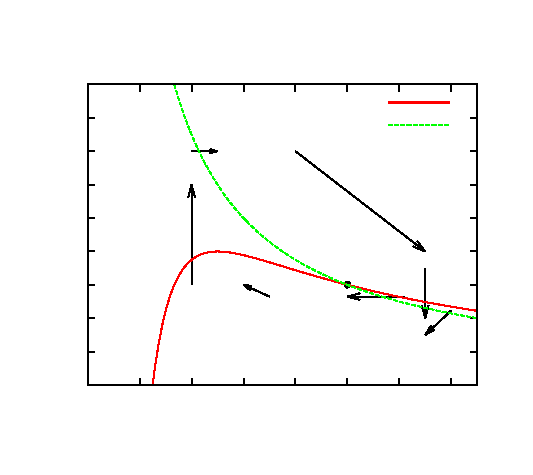
\includegraphics{trappingreg}}%
    \gplfronttext
  \end{picture}%
\endgroup
 %when using epslatex with gnuplot, make sure both the .tex
\caption[Trapping-Region]{Charakterisierung der Trapping-Region}
\label{fig:trapping}    % and .eps file are present
\end{center} 
 \end {figure}
\item Die Jacobi-Matrix am Fixpunkt lautet\begin{align*} \begin{bmatrix} -(b+1) + 2ayx & ax^2 \\ b-2ayx & -ax^2 \end{bmatrix}_{(x^*,y^*)} = \begin{bmatrix} b-1 & a \\ -b &  -a\end{bmatrix} =: A. \end{align*}
Damit ist $\trace(A) = b-(1+a)$ und $\det(A) = a > 0,$ weil $a > 0$ angenommen wurde. Da die Determinante gr\"o\ss er 0 ist, ist der Fixpunkt schon mal kein Sattel. Ist $\trace(A) < 0 \iff b < 1+a$ liegt Stabilit\"at  und f\"ur $b = 1+a$ ein lin. Zentrum vor. Falls $\trace(A) > 0$ ist, so ist er ein \emph{repeller}, d.h. ein instabiler Punkt oder eine instabile Spirale. Der kritische Wert ist also \begin{align}\label{exi} \trace(A) = b-(1+a) > 0 \iff b > 1+a =: b_{\mathrm{crit}}.\end{align}
\item Gilt nun \eqref{exi}, dann folgt mit dem Satz von Poincar\'e-Bendixson, dass es einen geschlossenen Orbit irgendwo in der Trapping-Region gibt, d.h. ein Grenzzyklus existiert f\"ur $b > b_{\mathrm{crit}}.$
\item Die Frequenz wird berechnet durch den Imagin\"arteil der EWe an der Bifurkation. Die EWe errechnet man mittels $\lambda^2 - \trace(A)\lambda + \det(A) = 0$ und weil f\"ur $b = b_{\mathrm{crit}}$, d.h. an der Bifurkation $\trace(A) = 0$ und $\det(A) > 0$ gelten, folgt, dass $\lambda_{1,2} =\pm i\sqrt{\det(A)} = \pm i \sqrt{a}. $ Damit ist die Periode gegeben durch \begin{equation*} \phi \approx \frac{2\pi}{\sqrt{a}}. \end{equation*}
\end{enumerate}
\end{loes}

\bigskip
\hrule
\begin{flushright}
\end{flushright}

%%%%%%%%%%%%%%%%%%%%%%%%%%%%%%%%%%%%%%%%%%%%%%%%%%%%%%%%%%%%%%%%%%%%%%%%%%%%%%%%

\end{document}
